% This work is licensed under the Creative Commons
% Attribution-NonCommercial-ShareAlike 4.0 International License. To view a copy
% of this license, visit http://creativecommons.org/licenses/by-nc-sa/4.0/ or
% send a letter to Creative Commons, PO Box 1866, Mountain View, CA 94042, USA.

\subsection{Triangulation}

%\Large{ $B_h$ oder $B_b$ ???}

\begin{definition_}
	Let $\Omega \subset \R^d$ ($d \geq 1$) bounded domain. A partition $T_h$ of $\Omega$ with $\tau \in T_h$ is a \textit{triangulation} if
	\begin{enumerate}[label=\alph*)]
		\item $\forall \tau \in T_h$, $\tau$ is closed, $\tau^0 \neq \emptyset$, $\tau$ is connected and $\partial \tau \in C^{0,1}$
		\begin{figure}[h!]
	\center

	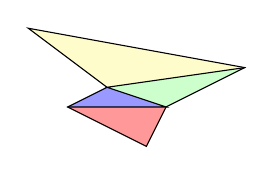
\begin{tikzpicture}[scale=1]
	
	
	% fill triangles
	\fill[red!40!white]   (0,0) -- ++(1,-0.5) -- ++(0.25,0.5) --cycle;
	\fill[blue!40!white]  (0,0) -- ++(1.25,0) --++(-0.75,0.25) --cycle;
	\fill[green!20!white]   (1.25,0) --++(-0.75,0.25) --++(1.75,0.25) --cycle;
	\fill[yellow!20!white]   (0.5,0.25) --++(1.75,0.25) --  ++(-2.75,0.5) --cycle;
	
	% outline
	\draw (0,0) -- ++(1,-0.5) -- ++(0.25,0.5)-- ++(1,0.5) -- ++(-2.75,0.5)-- ++(1,-0.75)--cycle;
	
	% this is unrobust
	\draw (0,0) -- ++(1.25,0) --++(-0.75,0.25) --++(1.75,0.25);
	
 	%\node at (1,-1) {example triangulation,};
	%\node at (1,-1.4) {$\tau$ disjunct};
	\end{tikzpicture}
		
\caption{example triangulation, $\tau$ disjunct}
\label{ch2_example_triang}

\end{figure}		
		\item $\bigcup \limits_{\tau \in T_h} = \overline{\Omega}$
		
		\item $\forall \tau_1,\tau_2 \in T_h:$ $\tau^0_1\cap \tau^0_2 = \emptyset$
	\end{enumerate}

	\begin{align*}
		h_{\tau} &= \diam (\tau)\\
		h &= \underset{\tau \in T_h}{\max} h_{\tau}\\
		\rho_{\tau} &= \underset{\tau \in T_h}{\sup} \{2r: B_r \subset \tau, d\text{-ball of radius  }r \} \\
		\rho &= \underset{\tau \in T_h}{\max} \rho_{\tau}
	\end{align*}
\end{definition_}
%TODO add picture

We further require that all faces of $\tau_i \in T_h$ are faces of $\tau_i \in T_h$ or part of $\partial \Omega$.
\begin{figure}[h!]
	\center


	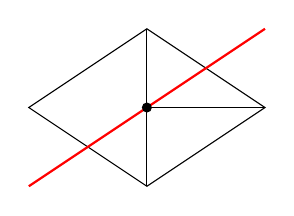
\begin{tikzpicture}[scale=1]

	% outline
	\draw (0,0) -- ++(1.5,-1) -- ++(1.5,1)-- ++(-1.5,1) -- cycle;
	\draw (1.5,-1) -- ++(0,2);
	\draw (1.5,0) -- ++(1.5,0);
	
	% red cross
	\draw[thick,red] (0,-1) --++ (3,2);

	% dot middle
	\filldraw (1.5,0) circle (1.6pt);

	\end{tikzpicture}

	\caption{not allowed}
	\label{ch1_triang_not_allowed}

\end{figure}
Hanging nodes cannot guarantee continuity of functions.

\begin{itemize}
	\item $T_h$ triangulation of $\Omega$ with Lagrange elements $(\tau,P_\tau,\Sigma_\tau)$ with $\tau \in T_h$
	\item  $N_h$ is set of all vertices of $T_h$. For $b\in N_0 $ $T_h(b) $ is the set of all finite elements, for which $b$ is a vertex.
\end{itemize}

\begin{definition_}
	(Finite elements space)
	\begin{equation*}
		X_h = \left \{ v = (v_\tau)_{\tau \in T_h} \in \prod \limits_{\tau \in T_h} P_\tau \left|
\begin{array}{c}
\forall b  \in\N_h : \forall \tau_1,\tau_2 \in T_h(b):\\
B_{b,\tau_1}(v_{\tau_1}) = B_{b,\tau_2}(v_{\tau_2}) 
\end{array}		
 \right.\right \}
	\end{equation*}
\end{definition_}
For Lagrange elements:
\begin{equation*}
	v_{\tau_1}(b) = B_{b,\tau_1}(v_{\tau_1}) = B_{b,\tau_2}(v_{\tau_2}) = v_{\tau_2}(b)
\end{equation*}

Functions on $X_h$ are uniquely determined by $\{v(b): b \in N_h \}$ we thus also have 
\begin{align*}
	X_h = \Big \{& v: \overline{\Omega} \to \R,\ \forall \tau \in T_h, v|_\tau \in P_\tau \text{ and }\\ &{} \quad \forall b \in N_h: \forall \tau_1,\tau_2 \in T_h(b) ,\ B_{b,\tau_1}(v|_{\tau_1}) = B_{b,\tau_2}(v|_{\tau_2})  \Big\}.
\end{align*}

\begin{example}
	linear lagrange elements $a_i$ vertex of $\tau \in T_h$,
	\begin{align*}
		B_{i,\tau}(p)  &= p(a_i) \quad \forall p \in P_\tau \\
		X_h &= \{ v:\overline{\Omega} \to \R : \forall \tau \in T_h, v|_{\tau} \in P_1(\tau) ,\ v \text{ continuous in } \overline{\Omega} \}
	\end{align*}
\end{example}

$X_h$ is a finite dimensional space, has a basis
\begin{equation*}
	\Sigma_h = \{ B_{h,j} : j= 1,\dots,N  \} \quad \text{ set of DoFs} 
\end{equation*}


\begin{itemize}
	\item $\varphi_i \in X_h$, $ i=1,\dots,N$ with
	\item  $B_{h,j}(\varphi_i) = \delta_{ij} \quad i,j=1,\dots,N$ (global basis funktions),
	\item $\varphi_i \in C^0(\overline{\Omega})$,
	\item  $\forall \tau \in T_h: \varphi_i|_\tau \in P_i(\tau)$.
	\item $\varphi_i(b_j) = \delta_{ij}$ for $i,j = 1,\dots,N$ with 
	\item $b_j \in N_h$ vertices of all $\tau \in T_h$.
\end{itemize}

\begin{tabular}{c|c}
	global  & local \\ \hline 
	&\\
	$\overline{\Omega} $&  ($\tau , P_\tau, \Sigma_\tau$) \\
	$X_h$ & $P_\tau = \{ v|_\tau :v \in X_h  \}$ \\
	global basis $\varphi_1,\dots,\varphi_N$ & local basis $p_1,\dots,p_N$ on $\tau$\\
	$\Sigma_h$ Dofs on $X$ & $\Sigma_\tau$ DoFs on $\tau$\\
	$b_1,\dots,b_N$ vertices of $\overline{\Omega}$ & $a_1,\dots,a_N$ vertices on $\tau$		
\end{tabular}
%%%TODO fix distances 

\begin{example}
	\begin{align*}
		- \laplace u &=1 \quad \tin \overline{\Omega} \subset \R\\
		u &=0 \quad \ton \partial \Omega
	\end{align*}
	\begin{equation*}
		a(u,v) = \int \limits_\Omega  \nabla u \cdot \nabla v \diff c = \int \limits_\Omega v\diff x = F(v) \quad \forall v \in H^1_0(\Omega)
	\end{equation*}
	\begin{align*}
		V_h &= \{ u \in X_h, u=0 \ton \partial \Omega  \}\\
			&= \{ u: \overline{\Omega} \to \R , \ u \text{ piecewise linear }, u=0 \ton \partial \Omega   \}
	\end{align*}
	$\varphi_1,\dots,\varphi_N$ global basis functions of $V_h$.
	\begin{equation*}
		a(\varphi_i,\varphi_j) = \int \limits_\Omega \nabla \varphi_i \cdot \nabla \varphi_j = 
		\begin{cases}
		\text{const} & \text{ if } a_i,a_j \text{ in some triangle}\\
		0 & \text{otherwise}
		\end{cases}
	\end{equation*}
	$\Omega = (-1,1)^2$, $h = \frac{1}{2}$.
	\begin{figure}[h!]
	\center
	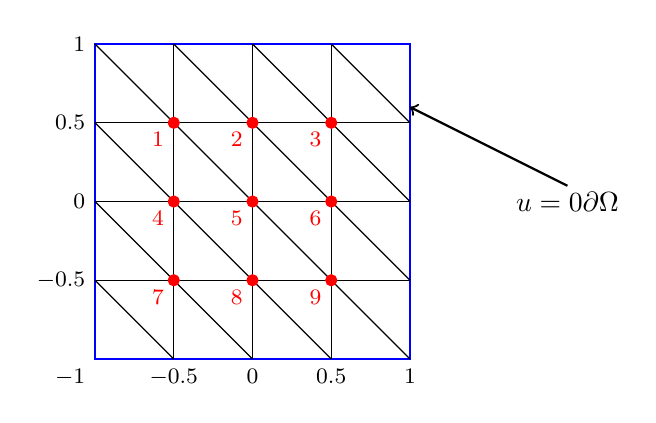
\begin{tikzpicture}[scale=2]
	
	\pgfmathsetmacro{\zerox}{-1}
	\pgfmathsetmacro{\zeroy}{-1}
	
	\draw[blue] (\zerox,\zeroy) -- ++(2,0)-- ++(0,2) --++(-2,0) --cycle;
	
	%vertical lines
	\draw (\zerox,\zeroy) ++(0.5,0)-- ++(0,2);
	\draw (\zerox,\zeroy) ++(1,0)-- ++(0,2);
	\draw (\zerox,\zeroy) ++(1.5,0)-- ++(0,2);
	
	% horizontal lines
	\draw (\zerox,\zeroy) ++(0,0.5)-- ++(2,0);
	\draw (\zerox,\zeroy) ++(0,1)-- ++(2,0);
	\draw (\zerox,\zeroy) ++(0,1.5)-- ++(2,0);
	
	% diagonal lines
	\draw (\zerox,\zeroy) ++(0,0.5)-- ++(0.5,-0.5);
	\draw (\zerox,\zeroy) ++(0,1)-- ++(1,-1);
	\draw (\zerox,\zeroy) ++(0,1.5)-- ++(1.5,-1.5);
	\draw (\zerox,\zeroy) ++(0,2)-- ++(2,-2);
	\draw (\zerox,\zeroy) ++(0.5,2)-- ++(1.5,-1.5);
	\draw (\zerox,\zeroy) ++(1,2)-- ++(1,-1);
	\draw (\zerox,\zeroy) ++(1.5,2)-- ++(0.5,-0.5);
	
	
	% inner points
	\filldraw[red]  (\zerox,\zeroy) ++ (0.5,0.5) circle (1pt)
					(\zerox,\zeroy) ++ (0.5,1) circle (1pt)
					(\zerox,\zeroy) ++ (0.5,1.5) circle (1pt)
					(\zerox,\zeroy) ++ (1,0.5) circle (1pt)
					(\zerox,\zeroy) ++ (1,1) circle (1pt)
					(\zerox,\zeroy) ++ (1,1.5) circle (1pt)
					(\zerox,\zeroy) ++ (1.5,0.5) circle (1pt)
					(\zerox,\zeroy) ++ (1.5,1) circle (1pt)
					(\zerox,\zeroy) ++ (1.5,1.5) circle (1pt);
	
	
	
	\fill[red,font=\footnotesize] (\zerox,\zeroy) ++ (0.5,1.5)  node[below left] {$1$}
								  (\zerox,\zeroy) ++ (1,1.5)  node[below left] {$2$}
								  (\zerox,\zeroy) ++ (1.5,1.5)  node[below left] {$3$}
								  (\zerox,\zeroy) ++ (0.5,1)  node[below left] {$4$}
								  (\zerox,\zeroy) ++ (1,1)  node[below left] {$5$}
								  (\zerox,\zeroy) ++ (1.5,1)  node[below left] {$6$}
								  (\zerox,\zeroy) ++ (0.5,0.5)  node[below left] {$7$}
								  (\zerox,\zeroy) ++ (1,0.5)  node[below left] {$8$}
								  (\zerox,\zeroy) ++ (1.5,0.5)  node[below left] {$9$};
	
	
	% axis numbering
	\fill[black,font=\footnotesize] (\zerox,\zeroy)  node[below left] {$-1$}
									(\zerox,\zeroy) ++(0.5,0) node[below] {$-0.5$}
									(\zerox,\zeroy) ++(1,0) node[below] {$0$}
									(\zerox,\zeroy) ++(1.5,0) node[below] {$0.5$}
									(\zerox,\zeroy) ++(2,0) node[below] {$1$}
									
									(\zerox,\zeroy) ++(0,0.5) node[left] {$-0.5$}
									(\zerox,\zeroy) ++(0,1) node[left] {$0$}
									(\zerox,\zeroy) ++(0,1.5) node[left] {$0.5$}
									(\zerox,\zeroy) ++(0,2) node[left] {$1$};
									
   	\node at (\zerox + 3,\zeroy + 1) {$u=0 \ton \partial \Omega$};
   	\draw[thick,-to] (\zerox + 3 ,\zeroy + 1.1) -- ++(-1,0.5);							    
	
	\end{tikzpicture}
		
	\caption{meshed $\Omega $}\label{tikz/chapter2/mesh_omega}
	\label{ch2_mesh_omega}

\end{figure}\\
	Define $F$ as follows
	\begin{align*}
		&{} F\colon \hat{\tau} \to \tau \quad F(x,y) = h \begin{pmatrix} x\\ y \end{pmatrix} + a_1\\
		&{} F^{-1}\colon \tau \to \hat{\tau} \quad F^{-1}(x,y) = h^{-1} \left ( \begin{pmatrix}x \\ y \end{pmatrix} - a_1 \right )
	\end{align*}
	
	
\begin{figure}[H]
	\center
	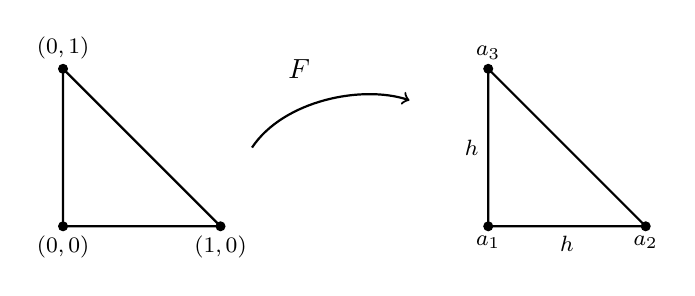
\begin{tikzpicture}[scale=2]
	
	
	% first simplex
	\draw[thick] (0,0) -- ++(0,1) -- ++(1,-1)--cycle;
	\filldraw (0,0)         circle (0.8pt)
			  (0,0) ++(1,0) circle (0.8pt)
			  (0,0) ++(0,1) circle (0.8pt);
	\fill[black,font=\footnotesize] (0,0) node[below] {$(0,0)$}
									(0,0) ++(1,0) node[below] {$(1,0)$}
									(0,0) ++(0,1) node[above] {$(0,1)$};
	
	%arrow
	\draw[thick,-to] (1.2,0.5) .. controls (1.4,0.8) and (1.9,0.9) .. (2.2, 0.8);
	
	%second simplex							
	\draw[thick] (0,0) ++ (2.7,0) -- ++(0,1) -- ++(1,-1)--cycle;
	\filldraw 	(0,0) ++ (2.7,0)         circle (0.8pt)
				(0,0) ++ (2.7,0) ++(1,0) circle (0.8pt)
				(0,0) ++ (2.7,0) ++(0,1) circle (0.8pt);
	%\filldraw (2.2,0)         circle (0.8pt)
	%		  (2.2,0) ++(2,0) circle (0.8pt)
	%		  (2.2,0) ++(1,1) circle (0.8pt);
	\fill[black,font=\footnotesize] (2.7,0) node[below] {$a_1$}
									(2.7,0) ++(1,0) node[below] {$a_2$}
									(2.7,0) ++(0,1) node[above] {$a_3$};								
			
	
	
	%\draw (2.2,0) ++(45:.6) arc (45:0:.6);
	
	
	\node at (1.5,1) {$F$};
	\fill[black,font=\footnotesize] (3.2,0)  node[below] {$h$}
									(2.7,0.5) node[left] {$h$};
	\end{tikzpicture}
	
	\caption{$F:\hat{\tau} \to \tau $}
	\label{ch2_plot_f}
	
\end{figure}
	
	\begin{align*}
		&\text{basis functions on } \hat{\tau} &&  \text{ basis functions on } \tau\\
		&\begin{rcases}
		&\hat{P}_1(x,y)=1-x-y \\
		&\hat{P}_2(x,y)=x \\
		&\hat{P}_3(x,y)=y \\
		\end{rcases}  \text{ for } (\hat{x},\hat{y}) \in \hat{\tau} \implies &&
		\begin{cases}
		P_1(x,y) = 1- \frac{x-x_1}{h} - \frac{y-y_1}{h} \\
		P_2(x,y) = \frac{x-x_1}{h} \\
		P_3(x,y) = \frac{y-y_1}{h} \\
		\end{cases}
	\end{align*}
	implies 
	\begin{equation*}
		A_{ij} =(a(\varphi_i, \varphi_j)) \in \R^{9 \times 9} 
	\end{equation*}
	
	\begin{figure}[h!]
	\center
	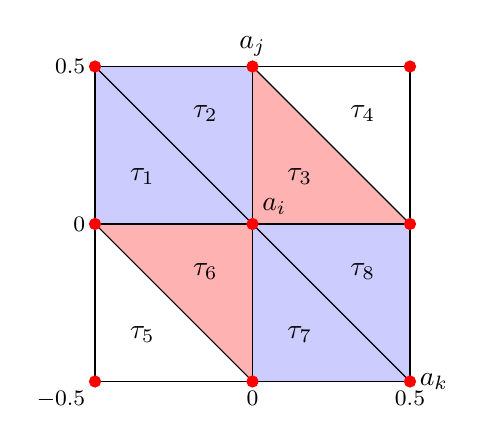
\begin{tikzpicture}[scale=2]
	
	\pgfmathsetmacro{\zerox}{-1}
	\pgfmathsetmacro{\zeroy}{-1}
	
	%color the important triangles
	\fill[red!30!] (\zerox,\zeroy) ++ (1,1) -- ++(0,-1) -- ++(-1,+1) --cycle;
	\fill[red!30!] (\zerox,\zeroy) ++ (1,1) -- ++(0,1) -- ++(1,-1) --cycle;
	
	\fill[blue!20!] (\zerox,\zeroy) ++ (1,1) -- ++(-1,0) -- ++(0,+1) -- ++(1,0) --cycle;
	\fill[blue!20!] (\zerox,\zeroy) ++ (1,1) -- ++(1,0) -- ++(0,-1) -- ++(-1,0) --cycle;
	
	% draw outline
	\draw (\zerox,\zeroy) -- ++(2,0)-- ++(0,2) --++(-2,0) --cycle;
	
	%vertical lines
	\draw (\zerox,\zeroy) ++(1,0)-- ++(0,2);
	
	% horizontal lines
	\draw (\zerox,\zeroy) ++(0,1)-- ++(2,0);

	
	% diagonal lines
	\draw (\zerox,\zeroy) ++(0,1)-- ++(1,-1);
	\draw (\zerox,\zeroy) ++(0,2)-- ++(2,-2);
	\draw (\zerox,\zeroy) ++(1,2)-- ++(1,-1);
	
	
	% inner points
	\filldraw[red]  (\zerox,\zeroy) circle (1pt)
					(\zerox,\zeroy) ++ (0,1) circle (1pt)
					(\zerox,\zeroy) ++ (0,2) circle (1pt)
					(\zerox,\zeroy) ++ (1,0) circle (1pt)
					(\zerox,\zeroy) ++ (1,1) circle (1pt)
					(\zerox,\zeroy) ++ (1,2) circle (1pt)
					(\zerox,\zeroy) ++ (2,0) circle (1pt)
					(\zerox,\zeroy) ++ (2,1) circle (1pt)
					(\zerox,\zeroy) ++ (2,2) circle (1pt);
	
	
	% number triangles
	\fill[black] (\zerox,\zeroy) ++ (0.3,1.3) node[] {$\tau_1$}
				 (\zerox,\zeroy) ++ (0.7,1.7)  node[] {$\tau_2$}
				 (\zerox,\zeroy) ++ (1.3,1.3)  node[] {$\tau_3$}
				 (\zerox,\zeroy) ++ (1.7,1.7)  node[] {$\tau_4$}
				 (\zerox,\zeroy) ++ (0.3,0.3)  node[] {$\tau_5$}
				 (\zerox,\zeroy) ++ (0.7,0.7)  node[] {$\tau_6$}
				 (\zerox,\zeroy) ++ (1.3,0.3)  node[] {$\tau_7$}
				 (\zerox,\zeroy) ++ (1.7,0.7)  node[] {$\tau_8$};

	
	
	% axis numbering
	\fill[black,font=\footnotesize] (\zerox,\zeroy)  node[below left] {$-0.5$}
									(\zerox,\zeroy) ++(1,0) node[below] {$0$}
									(\zerox,\zeroy) ++(2,0) node[below] {$0.5$}
									
									(\zerox,\zeroy) ++(0,1) node[left] {$0$}
									(\zerox,\zeroy) ++(0,2) node[left] {$0.5$};
									
	\fill[black] (\zerox,\zeroy) ++(1,1)  node[above right] {$a_i$}
				 (\zerox,\zeroy) ++(1,2)  node[above] {$a_j$}
   				 (\zerox,\zeroy) ++(2,0)  node[right] {$a_k$};

	
	\end{tikzpicture}
		
	\caption{important $\tau $}\label{tikz/chapter2/important_tau}
	\label{ch2_important_tau}

\end{figure}
	
	and 9 DoFs. As $\varphi_i = P^\tau_i$ in $\tau \in T_h(a_i)$
	\begin{align*}
		a(\varphi_i, \varphi_i) &= \displaystyle \sum^8_{i=1} \int \limits_{\tau_i} |\nabla \varphi_i|^2 \diff x\\
		&= 2 \int \limits_{\tau_3 } |\nabla P_1|^2 \diff x + 4 \int \limits_{\tau_i} |\nabla P_2|^2 \diff x\\
		&= 2 \frac{2}{h^2} \underbrace{\meas(\tau_3)}_{=\frac{h^2}{2}}  +4 \frac{1}{h^2} \underbrace{\meas(\tau_i)}_{=\frac{h^2}{2}}\\
		&=4
	\end{align*}
	 We will see that
	 \begin{align*}
	 	a(\varphi_i,\varphi_j) &= \dots = -1\\
	 	a(\varphi_i,\varphi_k) &= \dots = 0\\
	 \end{align*}
	 and thus 
	 \begin{equation*}
	 	A = \begin{pmatrix}
	 	0&-1&0\\
	 	-1&4&-1\\
	 	0&-1&0
	 	\end{pmatrix}
	 \end{equation*}
	
\end{example}

\section{Mesh Adaptivity for the FEM}
\subsection{Motivation and general concept}

\begin{example}
	poisson equation, uniform mesh, linear polinomials
\end{example}
\begin{center}
	\begin{tabular}{c | c}
		\underline{Quality} & \underline{Complexity}\\
		higher mesh resolution & higher mesh resolution requires \\
		$\to$ better approximation & additional computaional effort\\
		&  \\
		convergence & linear system \\
		$\|u-u_h\|_{L^2} \leq C h^2$ & $N_{\text{DoF}}\propto h^{-2}$
	\end{tabular}
\end{center}

Consens: Use fine meshes in regions with high gradient(something happens) and coarse meshes in regions with nearly constant gradiants(nothing happening)\\

Questions:
\begin{itemize}
	\item Where?\\
		\textit{prescribed} (with prior knowledge of the problem) or \\
		\textit{adaptive}(with error estimates,...)
	\item How?\\
		\textit{Red-Green Refinement} or \\
		\textit{Bisection}(we will only deal with this method here)
\end{itemize}

Method of Bisection:
\begin{itemize}
	\item define a refinemnt edge
	\item insert node in the middle
	\item replace old triangle wlth 2 new ones 
\end{itemize}
\begin{figure}[h!]
	\center
	\begin{tikzpicture}[scale=1]
	\def \xone{0};
	\def \yone{0};
	\def \h{3};
	
	% first triangle
	\coordinate (A) at (\xone,\yone);
	\coordinate (B) at ($ (A) + (\h,0) $);
	\coordinate (C) at ($ (A) + (\h/3,2*\h/3) $);
	\coordinate (M) at ($ (A) + (\h/2,0) $);

		
	\draw (A) -- (B) -- (C) --cycle;
	\filldraw (A) circle (1pt)
			  (B) circle (1pt)
			  (C) circle (1pt)
			  (M) circle (1pt);
	
	\draw[-to] (\h,\h/3) -- ++(\h/2,0);
	
	
	% first triangle
	\coordinate (A1) at (\xone +1.7*\h,\yone);
	\coordinate (B1) at ($ (A1) + (\h,0) $);
	\coordinate (C1) at ($ (A1) + (\h/3,2*\h/3) $);
	\coordinate (M1) at ($ (A1) + (\h/2,0) $);


	\draw (A1) -- (B1) -- (C1) --cycle;
	\draw (M1) -- (C1);
	\filldraw (A1) circle (1pt)
			  (B1) circle (1pt)
			  (C1) circle (1pt)
			  (M1) circle (1pt);
	 
	\end{tikzpicture}
	
	\caption{bisection refinement}\label{tikz/chapter_mesh/bisection_refine}
	\label{ch_m_bisection_refine}
	
\end{figure}

Shape regularity:
\begin{center}
	\begin{tabular}{c | c}
		\underline{mathmatical} & \underline{geometric}\\
		$\tau_h$:  triangulation & triangles not strongly stretched \\
		$h_T$:  diameter of $T$ & all angles should be \glqq simialar \grqq \\
		$\rho_T$:  radius of inscribed circle:	& gives the same qualitative description\\
		$\exists C > 0\ \forall T \in \tau_h \colon \rho_T \geq C h_T$ & 
	\end{tabular}
\end{center}
\begin{figure}[H]
	\center
	\begin{tikzpicture}[scale=1]
	\def \xone{0};
	\def \yone{0};
	\def \h{3};
	\def \r{2*\h/9 +\h*0.025}; % nicht schön, aber funktioniert
	
	% first triangle
	\coordinate (A) at (\xone,\yone);
	\coordinate (B) at ($ (A) + (\h,0) $);
	\coordinate (C) at ($ (A) + (\h/2,2*\h/3) $);
	\coordinate (M) at ($  (A) + (\h/2,\r)  $);
		
	\draw (A) -- (B) -- (C) --cycle;
	\draw[red] (A) -- (B);
	\draw[blue] (A) ++(\h/2,0) -- (M);
	\draw (M) circle (\r);
	\filldraw (A) circle (0.8pt)
			  (B) circle (0.8pt)
			  (C) circle (0.8pt)
			  (M) circle (0.8pt);
			  
	
	\def \ra{\h/13}; % nicht schön, aber funktioniert
	% second triangle
	\coordinate (D) at ($ (A) +(2*\h,0) $);
	\coordinate (E) at ($ (D) + (2*\h,0) $);
	\coordinate (F) at ($ (D) + (1*\h,\h/6) $);
	\coordinate (M2) at ($  (D) + (\h,\ra)  $);
	
	\draw (D) -- (E) -- (F) --cycle;
	\draw (M2) circle (\ra);
	\filldraw (D) circle (0.8pt)
			  (E) circle (0.8pt)
			  (F) circle (0.8pt)
			  (M2) circle (0.8pt);
	

	\node[below left] at (\h/3,0) {$h_T$};
	\node[below right] at (\h/2,\r/2) {$\rho_T$};
%	\fill[black,font=\footnotesize] (3.2,0)  node[below] {$h$}
%									(2.7,0.5) node[left] {$h$};
	\end{tikzpicture}
	
	\caption{different shapes}
	\label{ch_m_shape_regularity}
	
\end{figure}

Refinement edge:
\begin{itemize}
	\item chose longest edge for refinement
	\item shape regularity of mesh either remains or gets better
\end{itemize}

Problem: Hanging nodes
\begin{figure}[H]
	\center
	\begin{tikzpicture}[scale=1]
	\def \xone{0};
	\def \yone{0};
	\def \h{3};
	
	% first rectangle
	\coordinate (A) at (\xone,\yone);
	\coordinate (B) at ($ (A) + (\h,0) $);
	\coordinate (C) at ($ (A) + (\h,0.7*\h) $);
	\coordinate (D) at ($ (A) + (0,0.7*\h) $);
	\coordinate (M) at ($ (A) + (\h/2,0.35*\h) $);


	\fill[red!20] (A) --(B) --(D) -- cycle;		
	\draw (A) -- (B) -- (C) --(D) --cycle;
	\draw (B) --(D);
	\filldraw (A) circle (1pt)
			  (B) circle (1pt)
			  (C) circle (1pt)
			  (D) circle (1pt)
			  (M) circle (1pt);
	
	\draw[-to] (11/10*\h,\h/3) -- ++(\h/2,0);
	
	
	% second rectangle
	\coordinate (A1) at (\xone + 1.75*\h,\yone);
	\coordinate (B1) at ($ (A1) + (\h,0) $);
	\coordinate (C1) at ($ (A1) + (\h,0.7*\h) $);
	\coordinate (D1) at ($ (A1) + (0,0.7*\h) $);
	\coordinate (M1) at ($ (A1) + (\h/2,0.35*\h) $);
	
	
	\fill[green!20] (A1) --(B1) --(D1) -- cycle;	
	\fill[red!20] (C1) --(B1) --(D1) -- cycle;	
	\draw (A1) -- (B1) -- (C1) --(D1) --cycle;
	\draw (B1) --(D1);
	\draw (A1) --(M1);
	\filldraw (A1) circle (1pt)
			  (B1) circle (1pt)
			  (C1) circle (1pt)
			  (D1) circle (1pt)
			  (M1) circle (1pt);
	 
	\end{tikzpicture}
	
	\caption{hanging nodes}
	\label{ch_m_hanging_nodes}
	
\end{figure}
Refinement of a single triangle leads to a hanging node that is forbidden.\\
Solution: rekursive Refinement
\begin{enumerate}[label= case \arabic*:]
	\item Hanging node is on the refinement edge of a adjacent triangle
	\begin{figure}[h!]
	\center
	\begin{tikzpicture}[scale=1]
	\def \xone{0};
	\def \yone{0};
	\def \h{3};
	
	% first rectangle
	\coordinate (A) at (\xone,\yone);
	\coordinate (B) at ($ (A) + (\h,0) $);
	\coordinate (C) at ($ (A) + (\h,0.7*\h) $);
	\coordinate (D) at ($ (A) + (0,0.7*\h) $);
	\coordinate (M) at ($ (A) + (\h/2,0.35*\h) $);


	\fill[green!20] (A) --(B) --(D) -- cycle;
	\fill[red!20] (C) --(B) --(D) -- cycle;			
	\draw (A) -- (B) -- (C) --(D) --cycle;
	\draw (B) --(D);
	\draw (A) --(M);
	\filldraw (A) circle (1pt)
			  (B) circle (1pt)
			  (C) circle (1pt)
			  (D) circle (1pt)
			  (M) circle (1pt);
	
	\draw[-to] (11/10*\h,\h/3) -- ++(\h/2,0);
	
	
	% second rectangle
	\coordinate (A1) at (\xone + 1.75*\h,\yone);
	\coordinate (B1) at ($ (A1) + (\h,0) $);
	\coordinate (C1) at ($ (A1) + (\h,0.7*\h) $);
	\coordinate (D1) at ($ (A1) + (0,0.7*\h) $);
	\coordinate (M1) at ($ (A1) + (\h/2,0.35*\h) $);
	
	
	\fill[green!20] (A1) --(B1) --(D1) -- cycle;	
	\fill[green!20] (C1) --(B1) --(D1) -- cycle;	
	\draw (A1) -- (B1) -- (C1) --(D1) --cycle;
	\draw (B1) --(D1);
	\draw (A1) --(M1);
	\draw (C1) --(M1);
	\filldraw (A1) circle (1pt)
			  (B1) circle (1pt)
			  (C1) circle (1pt)
			  (D1) circle (1pt)
			  (M1) circle (1pt);
	 
	\end{tikzpicture}
	
	\caption{hanging nodes: case 1}\label{tikz/chapter_mesh/hanging_nodes_c1}
	\label{ch_m_hanging_nodes_c1}
	
\end{figure}

	\item Hanging node is \textbf{not} on refinement edge
	\begin{figure}[h!]
	\center
	\begin{tikzpicture}[scale=1]
	\def \xone{0};
	\def \yone{0};
	\def \h{3};
	
	% first rectangle
	\coordinate (A) at (\xone,\yone);
	\coordinate (B) at ($ (A) + (1.5*\h,0) $);
	\coordinate (C) at ($ (A) + (1.5*\h,\h) $);
	\coordinate (D) at ($ (A) + (0,\h) $);
	\coordinate (M) at ($ (A) + (0.75*\h,0.5*\h) $);
	\coordinate (AD) at ($ (A) + (0,0.5*\h) $);
	\coordinate (CD) at ($ (A) + (0.75*\h,\h) $);
	\coordinate (BC) at ($ (A) + (1.5*\h,0.5*\h) $);
	\coordinate (MMC) at ($ (A) + (3/4*1.5*\h,0.75*\h) $);

	%draw
	\filldraw[red!20] (M) --(MMC) -- (BC);			
	\draw (A) -- (B) -- (C) --(D) --cycle;
	\draw (B) --(D);
	\draw (A) --(C);
	\draw (AD) --(BC);
	\draw (M) --(CD) -- (BC);
	\foreach \i in {A,B,C,C,D,M,AD,CD,BC,MMC}{
		\filldraw (\i) circle (1.5pt);
	}

	
	\draw[-to] (8/5*\h,\h/2) -- ++(\h/2,0);
	
	
	% second rectangle
	\coordinate (A1) at (\xone +  2.25*\h,\yone);
	\coordinate (B1) at ($ (A1) + (1.5*\h,0) $);
	\coordinate (C1) at ($ (A1) + (1.5*\h,\h) $);
	\coordinate (D1) at ($ (A1) + (0,\h) $);
	\coordinate (M1) at ($ (A1) + (0.75*\h,0.5*\h) $);
	\coordinate (AD1) at ($ (A1) + (0,0.5*\h) $);
	\coordinate (CD1) at ($ (A1) + (0.75*\h,\h) $);
	\coordinate (BC1) at ($ (A1) + (1.5*\h,0.5*\h) $);
	\coordinate (MMC1) at ($ (A1) + (3/4*1.5*\h,0.75*\h) $);
	\coordinate (MMBC1) at ($ (A1) + (3/4*1.5*\h,0.5*\h) $);
	
	%draw
	\fill[red!20] (M1) --(B1) --(BC1) -- cycle;
	\filldraw[green!20] (M1) --(MMC1) -- (BC1);			
	\draw (A1) -- (B1) -- (C1) --(D1) --cycle;
	\draw (B1) --(D1);
	\draw (A1) --(C1);
	\draw (AD1) --(BC1);
	\draw (M1) --(CD1) -- (BC1);
	\draw (MMC1) --(MMBC1);
	\foreach \i in {A1,B1,C1,C1,D1,M1,AD1,CD1,BC1,MMC1,MMBC1}{
		\filldraw (\i) circle (1.5pt);
	}

	\draw[-to] (\xone +  2.1*\h,\yone - 0.1*\h) -- ++(-\h/2,-\h/3);
	
	
	% third rectangle
	\coordinate (A2) at (\xone ,\yone -1.5*\h);
	\coordinate (B2) at ($ (A2) + (1.5*\h,0) $);
	\coordinate (C2) at ($ (A2) + (1.5*\h,\h) $);
	\coordinate (D2) at ($ (A2) + (0,\h) $);
	\coordinate (M2) at ($ (A2) + (0.75*\h,0.5*\h) $);
	\coordinate (AD2) at ($ (A2) + (0,0.5*\h) $);
	\coordinate (CD2) at ($ (A2) + (0.75*\h,\h) $);
	\coordinate (BC2) at ($ (A2) + (1.5*\h,0.5*\h) $);
	\coordinate (MMC2) at ($ (A2) + (3/4*1.5*\h,0.75*\h) $);
	\coordinate (MMBC2) at ($ (A2) + (3/4*1.5*\h,0.5*\h) $);
	\coordinate (MMB2) at ($ (A2) + (3/4*1.5*\h,0.25*\h) $);
	\coordinate (AB2) at ($ (A2) + (0.5*1.5*\h,0) $);
	
	
	%draw
	\fill[red!20] (M2) --(B2) --(BC2) -- cycle;
	\fill[red!20] (A2) --(B2) --(M2) -- cycle;
	\filldraw[green!20] (M2) --(MMC2) -- (BC2);			
	\draw (A2) -- (B2) -- (C2) --(D2) --cycle;
	\draw (B2) --(D2);
	\draw (A2) --(C2);
	\draw (AD2) --(BC2);
	\draw (M2) --(CD2) -- (BC2);
	\draw (MMC2) --(MMBC2);
	\foreach \i in {A2,B2,C2,D2,M2,AD2,CD2,BC2,MMC2,MMBC2,MMB2,AB2}{
		\filldraw (\i) circle (1.5pt);
	}

	\draw[-to] (8/5*\h,-\h) -- ++(\h/2,0);
	
	% fourth rectangle
	\coordinate (A3) at (\xone +  2.25*\h,\yone-1.5*\h);
	\coordinate (B3) at ($ (A3) + (1.5*\h,0) $);
	\coordinate (C3) at ($ (A3) + (1.5*\h,\h) $);
	\coordinate (D3) at ($ (A3) + (0,\h) $);
	\coordinate (M3) at ($ (A3) + (0.75*\h,0.5*\h) $);
	\coordinate (AD3) at ($ (A3) + (0,0.5*\h) $);
	\coordinate (CD3) at ($ (A3) + (0.75*\h,\h) $);
	\coordinate (BC3) at ($ (A3) + (1.5*\h,0.5*\h) $);
	\coordinate (MMC3) at ($ (A3) + (3/4*1.5*\h,0.75*\h) $);
	\coordinate (MMBC3) at ($ (A3) + (3/4*1.5*\h,0.5*\h) $);
	\coordinate (MMB3) at ($ (A3) + (3/4*1.5*\h,0.25*\h) $);
	\coordinate (AB3) at ($ (A3) + (0.5*1.5*\h,0) $);
	
	%draw
	\fill[red!20] (M3) --(MMB3) --(BC3) -- cycle;
	\fill[red!20] (AB3) --(B3) --(M3) -- cycle;
	\filldraw[green!20] (M3) --(MMC3) -- (BC3);	
	\filldraw[green!20] (B3) --(BC3) -- (MMB3);
	\filldraw[green!20] (A3) --(AB3) -- (M3);				
	\draw (A3) -- (B3) -- (C3) --(D3) --cycle;
	\draw (B3) --(D3);
	\draw (A3) --(C3);
	\draw (AD3) --(BC3);
	\draw (M3) --(CD3) -- (BC3);
	\draw (MMC3) --(MMBC3);
	\draw (BC3) --(MMB3);
	\draw (M3) --(AB3);
	\foreach \i in {A3,B3,C3,C3,D3,M3,AD3,CD3,BC3,MMC3,MMBC3,MMB3,AB3}{
		\filldraw (\i) circle (1.5pt);
	}
	
	\draw[-to] (\xone +  2.1*\h,\yone - 1.6*\h) -- ++(-\h/2,-\h/3);
	
	% fifth rectangle
	\coordinate (A4) at (\xone ,\yone -3*\h);
	\coordinate (B4) at ($ (A4) + (1.5*\h,0) $);
	\coordinate (C4) at ($ (A4) + (1.5*\h,\h) $);
	\coordinate (D4) at ($ (A4) + (0,\h) $);
	\coordinate (M4) at ($ (A4) + (0.75*\h,0.5*\h) $);
	\coordinate (AD4) at ($ (A4) + (0,0.5*\h) $);
	\coordinate (CD4) at ($ (A4) + (0.75*\h,\h) $);
	\coordinate (BC4) at ($ (A4) + (1.5*\h,0.5*\h) $);
	\coordinate (MMC4) at ($ (A4) + (3/4*1.5*\h,0.75*\h) $);
	\coordinate (MMBC4) at ($ (A4) + (3/4*1.5*\h,0.5*\h) $);
	\coordinate (MMB4) at ($ (A4) + (3/4*1.5*\h,0.25*\h) $);
	\coordinate (AB4) at ($ (A4) + (0.5*1.5*\h,0) $);
	
	
	%draw
	\fill[red!20] (M4) --(MMB4) --(BC4) -- cycle;
	\fill[red!20] (AB4) --(B4) --(M4) -- cycle;
	\filldraw[green!20] (B4) --(BC4) -- (MMB4);
	\filldraw[green!20] (M4) --(MMC4) -- (BC4);
	\filldraw[green!20] (A4) --(AB4) -- (M4);			
	\draw (A4) -- (B4) -- (C4) --(D4) --cycle;
	\draw (B4) --(D4);
	\draw (A4) --(C4);
	\draw (AD4) --(BC4);
	\draw (M4) --(CD4) -- (BC4);
	\draw (MMC4) --(MMBC4);
	\draw (BC4) --(MMB4);
	\draw (M4) --(AB4);
	\foreach \i in {A4,B4,C4,D4,M4,AD4,CD4,BC4,MMC4,MMBC4,MMB4,AB4}{
		\filldraw (\i) circle (1.5pt);
	}
	
	\draw[-to] (8/5*\h,-2.5*\h) -- ++(\h/2,0);
	
	% sixth rectangle
	\coordinate (A5) at (\xone +  2.25*\h ,\yone -3*\h);
	\coordinate (B5) at ($ (A5) + (1.5*\h,0) $);
	\coordinate (C5) at ($ (A5) + (1.5*\h,\h) $);
	\coordinate (D5) at ($ (A5) + (0,\h) $);
	\coordinate (M5) at ($ (A5) + (0.75*\h,0.5*\h) $);
	\coordinate (AD5) at ($ (A5) + (0,0.5*\h) $);
	\coordinate (CD5) at ($ (A5) + (0.75*\h,\h) $);
	\coordinate (BC5) at ($ (A5) + (1.5*\h,0.5*\h) $);
	\coordinate (MMC5) at ($ (A5) + (3/4*1.5*\h,0.75*\h) $);
	\coordinate (MMBC5) at ($ (A5) + (3/4*1.5*\h,0.5*\h) $);
	\coordinate (MMB5) at ($ (A5) + (3/4*1.5*\h,0.25*\h) $);
	\coordinate (AB5) at ($ (A5) + (0.5*1.5*\h,0) $);
	
	
	%draw
	\fill[green!20] (M5) --(MMB5) --(BC5) -- cycle;
	\fill[green!20] (AB5) --(B5) --(M5) -- cycle;
	\filldraw[green!20] (B5) --(BC5) -- (MMB5);
	\filldraw[green!20] (M5) --(MMC5) -- (BC5);
	\filldraw[green!20] (A5) --(AB5) -- (M5);			
	\draw (A5) -- (B5) -- (C5) --(D5) --cycle;
	\draw (B5) --(D5);
	\draw (A5) --(C5);
	\draw (AD5) --(BC5);
	\draw (M5) --(CD5) -- (BC5);
	\draw (MMC5) --(MMBC5);
	\draw (BC5) --(MMB5);
	\draw (M5) --(AB5);
	\draw (AB5) --(MMB5);
	\draw (MMB5) --(MMBC5);
	\foreach \i in {A5,B5,C5,D5,M5,AD5,CD5,BC5,MMC5,MMBC5,MMB5,AB5}{
		\filldraw (\i) circle (1.5pt);
	}
	
	\end{tikzpicture}
	
	\caption{hanging nodes: case 2}\label{tikz/chapter_mesh/hanging_nodes_c2}
	\label{ch_m_hanging_nodes_c2}
	
\end{figure}
	still better, than refining ehole domain\\
	$\implies$ multiple recursive refinements necessary
\end{enumerate}

\subsection{Data structures}
\underline{direct storage}
\begin{itemize}
	\item different array for nodes and cells(like in the tutorial)
	\begin{figure}[h!]
	\center
	\begin{tikzpicture}[scale=1]
	\def \xone{0};
	\def \yone{0};
	\def \h{3};
	
	% first rectangle
	\coordinate (1) at (\xone,\yone);
	\coordinate (2) at ($ (A) + (\h,0) $);
	\coordinate (3) at ($ (A) + (0,0.7*\h) $);
	\coordinate (4) at ($ (A) + (\h,0.7*\h) $);
	\coordinate (5) at ($ (A) + (\h/2,0.35*\h) $);

	\draw (1) -- (2) -- (4) --(3) --cycle;
	\draw (2) --(3);
	\foreach \i in {1,2}{
		\filldraw (\i) circle (1.5pt);
		\node[below]  at (\i) {\i};
	}
	\foreach \i in {3,4}{
		\filldraw (\i) circle (1.5pt);
		\node[above]  at (\i) {\i};
	}
	
	\end{tikzpicture}
	
	\caption{visualize data structure}\label{tikz/chapter_mesh/data_structure}
	\label{ch_m_data_structure}
	
\end{figure}
	\item cells = 
	$\begin{bmatrix}
		1 & 2 & 3\\
		4 & 3 & 2
	\end{bmatrix} $ (refinement edge is defined by the last 2 entries in corresponding line)
	
\end{itemize}
Bisections on direct storage:
\begin{itemize}
	\item additional node
	\item replace 1 cell by 2 cells
	\begin{figure}[H]
	\center
	\begin{tikzpicture}[scale=1]
	\def \xone{0};
	\def \yone{0};
	\def \h{3};
	
	% first rectangle
	\coordinate (1) at (\xone,\yone);
	\coordinate (2) at ($ (A) + (\h,0) $);
	\coordinate (3) at ($ (A) + (0,0.7*\h) $);
	\coordinate (4) at ($ (A) + (\h,0.7*\h) $);
	\coordinate (5) at ($ (A) + (\h/2,0.35*\h) $);

	\draw (1) -- (2) -- (4) --(3) --cycle;
	\draw (2) --(3);
	\draw (1) --(5);
	\foreach \i in {1,2}{
		\filldraw (\i) circle (1.5pt);
		\node[below]  at (\i) {\i};
	}
	\foreach \i in {3,4}{
		\filldraw (\i) circle (1.5pt);
		\node[above]  at (\i) {\i};
	}
	\filldraw (5) circle (1.5pt);
	\node[above]  at (5) {5};
	
	\end{tikzpicture}
	
	\caption{visualize bisection data structure}
	\label{ch_m_bisection_data_structure}
	
\end{figure}
	\item cells = 
	$\begin{bmatrix}
	5 & 1 & 2\\
	5 & 3 & 1\\
	4 & 3 & 2
	\end{bmatrix} $ (first index is the new node and the structure regarding the refinement edge stays)
	
\end{itemize}

Advantages:
\begin{itemize}
	\item minimal memory consumption
	\item simple implementation
	\item all information directly available
\end{itemize}

Disadvantages:
\begin{itemize}
	\item working on arrays: size-changes are costly computations
	\item coarsening of meshes is very difficult
	\item neighboring relatons have to be computed explicitly after every refinement
\end{itemize}
Thus not so good for moving regions of interest.
\vspace{1cm}

\underline{hierarchical storage}
\begin{itemize}
	\item start from a coarse \glqq macro mesh \grqq
	\item store all refonement steps not only the current mesh
	\item well suited dara structure: \textbf{binary tree}
\end{itemize}

short exkurs: binary trees\\
tree nodes:
\begin{itemize}
	\item pointer to $\leq 2$ children
	\item pointer to $\leq 1$ father
	\item data
	\tikzset
{
	treenode/.style = {circle, draw=blue!60, fill=blue!40, very thick, minimum size=4mm}
}

\begin{figure}[H]
	\center
	\begin{tikzpicture}[->,>=stealth', level/.style={sibling distance = 2cm/#1, level distance = 1.5cm}, scale=0.6,transform shape, scale = 1.5]
	\node [treenode] {}
	child
	{
		node [treenode] {} 
		child
		{
			node [treenode] {} 
			child
			{
				node [treenode] {} 
			}
			child
			{
				node [treenode] {} 
			}
		}
		child
		{
			node [treenode]  {}  
		}
	}
	child
	{
		node [treenode]  {}     
	};
	
	\end{tikzpicture}	
\end{figure}


	

	%%TODO pic
\end{itemize}
properties:
\begin{itemize}
	\item no father: \textit{root}
	\item no children: \textit{leaf}
\end{itemize}

Applications:
\begin{itemize}
	\item search tree: heap
	\item hierarchical mesh
\end{itemize}

hierarchical mesh tree:
Node:
\begin{itemize}
	\item pointer: father,children
	\item data: vertices of the represented mesh cell
\end{itemize}

Mesh:
\begin{itemize}
	\item macro mesh explicitly defined
	\item every macro mesh cell ist \underline{root} of a tree
	\item current mesh os given by all \underline{leafs}
	%%TODO add pic
\end{itemize}

Advantages:
\begin{itemize}
	\item large libraries for tree strictires already existent(computation of neighbors, etc.)
	\item coarsening is a trivial task(remove leafs)
	\item refinement inherited from father (determined by tree structure)(compute neighboring relations \glqq on demand\grqq)
	%%TODO add pic
\end{itemize}

Disadvantages:
\begin{itemize}
	\item memory consumption(storage of unnecessary nodes)
	\item high implementational effort
\end{itemize}

\subsection{Conclusion and Outlook}
\begin{enumerate}[label = \arabic* .]
	\item local mesh refinement can be a powerful tool to find the optimal balence between performance and accuracy
	\item prevention of hanging nodes requieres a recursive refinement strategy
	\item both datastructures have advantages and disadvantages  
\end{enumerate}
Open questions:
\begin{enumerate}[label = \arabic* .]
	\item Where to refine(explicitly give locations, error estimates,...)?
	\item How to prove that it actually works(convergence orders)?
	\item What could have been done differently?\\
	$\implies$ Replace Bisection- by Red-Green Refinement...\\
	$\implies$ $p$-Adaptivity instead of $h$-Adaptivity(take higher order polonomial basisfunctions)
\end{enumerate}



